\documentclass{llncs}
\usepackage{tikz}
\usetikzlibrary{shapes,arrows,calc}


%\usepackage{url}
\usepackage{multirow}
\usepackage{listings}
\usepackage{amsmath}  % for equation*
\usepackage{array}    % for tabular
\usepackage{verbatim} % for comment
\usepackage{wrapfig}
\usepackage[final]{microtype}
\usepackage[pdfborder={0 0 0}]{hyperref}
\usepackage{tabularx}

\newcommand\forAll[1]{\forall \, #1 \, . \,}
\newcommand\forAllII[2]{\forall \, #1 \, #2 \, . \,}

\newcommand\propno[1]{(\emph{#1})}
\newcommand\hs[1]{\texttt{#1}}

% \raggedbottom

\lstnewenvironment{code}[1][]
  {\noindent
   \vspace{-0.5\baselineskip}
   \lstset{basicstyle=\ttfamily,
           frame=single,
           language=Haskell,
           keywordstyle=\color{black},
           #1}
   \fontsize{8pt}{8pt}\selectfont}
  {}

\newcommand\NOTE[1]{} % \mbox{}\marginpar{\fontsize{8pt}{8pt}\selectfont\raggedright\hspace{0pt}\emph{#1}}}

\def\maindocument{} % To tell tikz images that they are not stand alone

\begin{document}

\title{Hipster: Integrating Theory Exploration in a Proof Assistant}

\author{Moa Johansson \and Dan Ros\'en \and Nicholas Smallbone \and Koen Claessen}
\institute{Department of Computer Science and Engineering, Chalmers University of Technology
	\email{\{jomoa,danr,nicsma,koen\}@chalmers.se}
	}

\authorrunning{Johansson, Ros\'en, Smallbone, Claessen}
\titlerunning{Integrating Theory Exploration in a Proof Assistant}

\maketitle

\begin{abstract}

This paper describes Hipster, a system integrating theory exploration with the proof assistant Isabelle/HOL. Theory exploration is a technique for automatically discovering new interesting lemmas in a given theory development.
Hipster can be used in two main modes. The first is {\em exploratory mode}, used for automatically generating basic lemmas about a given set of datatypes and functions in a new theory development. The second is {\em proof mode}, used in a particular proof attempt, trying to discover the missing lemmas which would allow the current goal to be proved. Hipster's proof mode complements and boosts existing proof automation techniques that rely on automatically selecting existing lemmas, by inventing new lemmas that need induction to be proved. We show example uses of both modes.
\end{abstract}

% removed from the abstract:
%Existing Isabelle-tools like Sledgehammer can automatically select existing lemmas from the libraries that are likely to be needed for automation of many proofs.

\section{Introduction}
\label{sec:intro}
The concept of theory exploration was first introduced by Buchberger \cite{buchberger2000theory}. He argues that as a contrast to  automated theorem provers that focus on proving one theorem at the time in isolation, mathematicians instead typically proceed by exploring entire theories, by conjecturing and proving layers of increasingly complex propositions. For each layer, appropriate proof methods are identified, and previously proved lemmas may be used to prove later conjectures. When a new concept (e.g. a new function) is introduced, we should prove a set of new conjectures which, ideally, "completely" relates the new with the old, after which other propositions in this layer can be proved easily by easy "routine" reasoning. Mathematical software should be designed to support this workflow. This is arguably what many interactive proof assistants, such as Theorema \cite{theorema} and Isabelle \cite{isabelle}, roughly support. However, they leave the generation of new conjectures relating different concepts largely to the user. Recently, a number of different systems have been implemented to address also this aspect of theory exploration \cite{McCasland2006,isacosy,isascheme,hipspecCADE}.  In this work, we take this one step further by integrating the discovery and proof of new conjectures in the workflow of the interactive theorem prover Isabelle. Our system, called Hipster, is based on our previous work on HipSpec \cite{hipspecCADE}, a theory exploration system for Haskell programs. In \cite{hipspecCADE} we showed that HipSpec is able to automatically discover many of the equational theorems present in Isabelle's list library. In this article we show how this can be used to speed up the development of new theories in Isabelle by discovering basic lemmas automatically. 
Isabelle theories are translated into Haskell, after which computation and evaluation in Haskell is used to efficiently generate generate interesting conjectures, which are then imported back into Isabelle and proved by automated tactics. Hipster can be used in two main ways: in \emph{exploratory mode} it quickly discovers basic properties about a newly defined function and its relationship to already existing ones. Hipster can also be used in \emph{proof mode}, to provide lemma hints for an ongoing proof attempt when the user is stuck. 

Our work also fits nicely with the increased popularity of Sledgehammer \cite{sledgehammer}, an Isabelle tool allowing the user to call various external automated provers. Sledgehammer use \emph{relevance filtering} to select among the available lemmas those likely to be useful for proving a given conjecture \cite{mash}. However, if a crucial lemma is missing, the proof attempt will fail. If theory exploration is employed before, we can increase the chances of Sledgehammer succeeding with little user effort. 

HERE: short example? Something unprovable by Sledgehammer before theory exploration.

%Hipster is parametrised by tactics for routine and "hard" reasoning. In this paper, we consider routine reasoning to be first-order resoning by Metis, give the conjectures Hipster has proved so far while "hard" reasoning is those proofs requiring induction. 

%Sledgehammer is a popular and powerful tool in Isabelle which allows users to call various external automated first-order provers \cite{sledgehammer}. Proofs are then replayed inside Isabelle's trusted kernel using its Metis prover. Sledgehammer's machine learning based relevance filter \cite{mash}, selects a number of facts from Isabelle's library that are judged to likely be relevant for the problem at hand. 
% 
%Which is because we can improve on Sledgehammer-style interactions in cases when the required lemmas simply are not available, so Sledgehammer would fail. 
Integrating the theory exploration system in an interactive setting has several other advantages, for instance when exploring a large theory which otherwise would generate a very large search space. The user can instead incrementally explore different relevant sub-theories while avoiding a search space explosion. Lemmas discovered in each sub-theory can be made available when exploring increasingly larger sets of functions. 

The article is organised as follows: In section \ref{sec:background} we give a brief overview of the HipSpec system which Hipster use to generate conjectures, after which we describe Hipster in more detail in section \ref{sec:hipster}. Blanchette variables in section X etc...


\section{Background}
\label{sec:background}

In this section we give a brief overview of the HipSpec system which
we use as a backend for generating conjectures. HipSpec is a
state-of-the-art inductive theorem prover and theory exploration
system for Haskell. In \cite{hipspecCADE} we showed that HipSpec is
able to automatically discover and prove the kind of equational lemmas present in
Isabelle's libraries, when given the corresponding functions written in Haskell.

HipSpec works in two stages:
\begin{enumerate}
\item Generate a set of conjectures about the functions at hand. These conjectures are equations between terms involving the given functions, and are only tested for correctness.

\item Attempt to prove each of the conjectures, using already proven conjectures as assumptions. HipSpec implements this by enumerating induction schemas, and firing off many proof obligations to automated first-order logic theorem provers.
\end{enumerate}
The proving power of HipSpec comes from its capability to
automatically discover and prove lemmas, which are then used to help
subsequent proofs.

In Hipster we are not interested in HipSpec's
proving capabilities (stage (2) above); we use Isabelle for the proofs instead. Isabelle
is based on a small core of trusted axioms, and proofs must be built
on top of those axioms. In other words, we would have to reconstruct
inside Isabelle any proof we found anyway, so it is easier to use
Isabelle for the proofs in the first place.

The part of HipSpec we do use
is its conjecture synthesis system (part (1) above), called QuickSpec \cite{quickspec}),
which efficiently generates equations about given functions and
datatypes.

QuickSpec takes a set of functions as input, and proceeds to generate all
type-correct terms up to a given limit (usually up to depth three), with
variables (usually three per type).  It first assumes that all terms the same
type are equivalent, and initially puts them in the same equivalence class.  By
generating random values for the variables (using QuickCheck \cite{quickcheck}), the terms are repeatedly evaluated and their equivalence
classes are separated according to the evaluation results.  This process is
repeated until the equivalence classes stabilise, and resulting equations can
be read off from each equivalence class.  This means that the conjectures
generated are, although not yet proved, fairly likely to be true.

As an example, we tell QuickSpec to explore the theory with list append,
\verb~@~, the empty list, \verb~[]~, and three list variables \verb~xs~,
\verb~ys~, \verb~zs~. Some of all the terms it will generate are these:
\verb~(xs@ys)@zs~, \verb~xs@(ys@zs)~, \verb~xs@[]~ and simply \verb~xs~.
Initially, all four will be assumed to be in the same equivalence class.
Before soon, it will generate non-empty lists for \verb~ys~ and \verb~zs~.
Evaluating the terms with such assignments will split this equivalence class
into two: one with the former two and one with the latter. After this, more
values will be generated for these lists variables, but no evaluation will make
them split again. Eventually, QuickSpec stops and the equations for
associativity and right identity can be read off.



\section{Hipster: Implementation and Use}
\label{sec:hipster}

In this section we give an overview of Hipster, and show how it can be used both in theory exploration mode and in proof mode, to find lemmas relevant for a particular proof attempt. An overview of Hipster is shown in figure \ref{fig:hipster}. The source code and examples are available online\footnote{\url{https://github.com/moajohansson/IsaHipster}}.

\begin{figure}[htbp]
\begin{center}
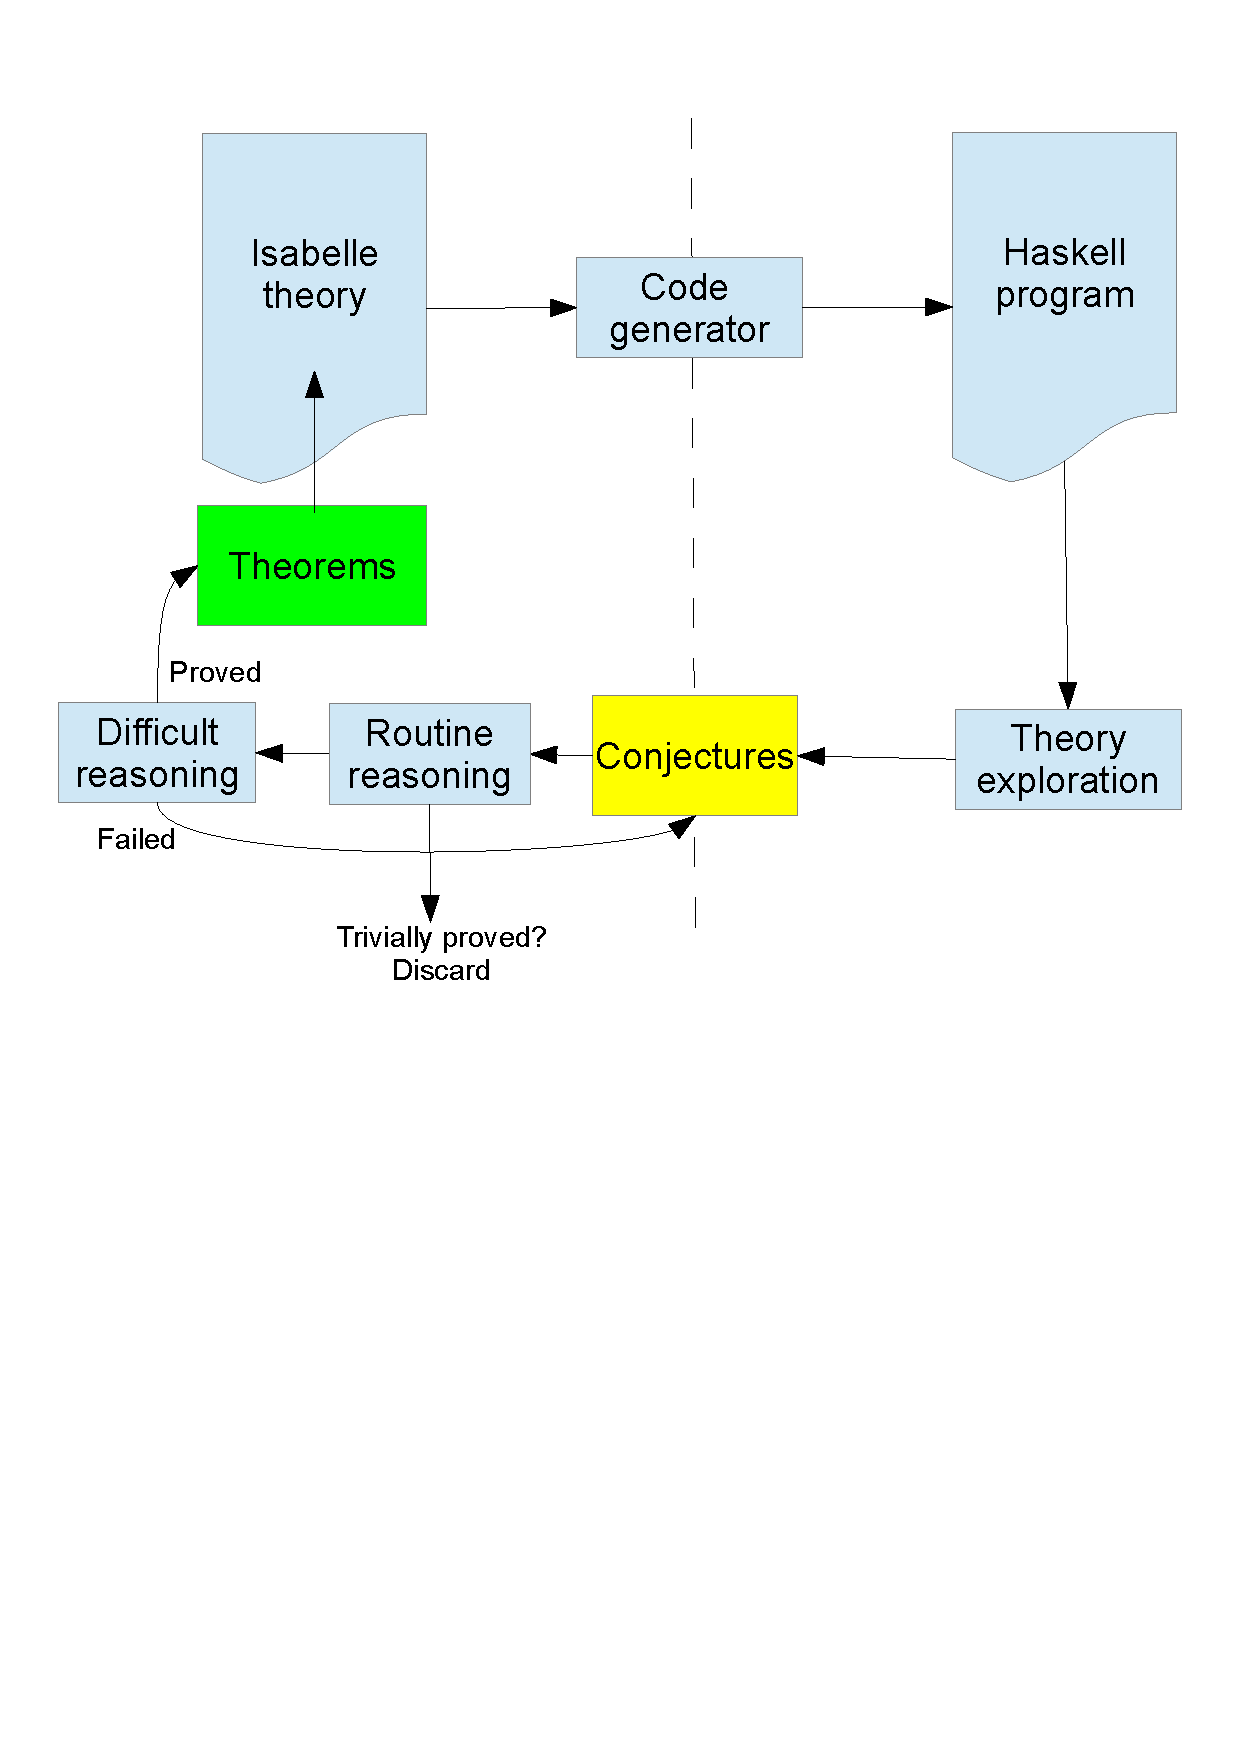
\includegraphics[scale=0.45]{hipster}

\caption{Overview of Hipster}
\label{fig:hipster}
\end{center}
\end{figure}

Starting from an Isabelle theory, Hipster calls Isabelle's code generator \cite{codegen} to translate the given functions into a Haskell program. In order to use the testing framework from QuickCheck, as described in the previous section, we must however also post-process the Haskell file, adding \emph{generators}, which are responsible for producing arbitrary values used for evaluation and testing. We use generators automatically deduced by the Feat package \cite{feat}. Another important issue that need to be addressed at this stage is the differences in semantics for partial functions in Isabelle and Haskell. In order to avoid HipSpec missing equations that hold in Isabelle, but not in Haskell, we had to modify the translation of partial functions. This is explained in more detail in section \ref{sec:partial}.

Once the Haskell program is in place, we run theory exploration and generate a set of equational conjectures, which HipSpec orders according to generality. More general equations are preferred, as we expect these to be more widely applicable as lemmas. In previous work on HipSpec, the system would at this stage apply induction on the conjectures and send them off to some external prover. Here, we instead import them back into Isabelle as we wish to produce checkable LCF-style proofs for our conjectures. 

The proof procedure in Hipster is parametrised by two tactics, one for easy or \emph{routine reasoning} and one for \emph{difficult reasoning}. In the examples below, we use Isabelle's simplifier followed by first-order reasoning by Metis \cite{metis} as routine reasoning, and a tactic performing structural induction followed by simplification and first-order reasoning as difficult reasoning. Metis is restricted to run for at most one second in both the routine and difficult tactic. If there are several possible variables to apply induction to, we may backtrack if the first choice fails. Both tactics have access to the theorems proved so far, and hence gets stronger as the proof procedure proceed through the list of conjectures. 

As there are rather many conjectures produced by theory exploration, we do not want to present them all to the user, but rather select the most interesting ones, which are difficult to prove. Those that follow only by routine reasoning are filtered out. 
Depending on the theory and application we can change these tactics to suit our needs. If we want Hipster to produce fewer or more lemmas, we can choose a stronger or weaker tactic, allowing for flexibility.  

The order in which Hipster tries to prove things matter. As we mentioned, it will try more general conjectures first, with the hope that they will be useful to filter out many more specific routine results. Occasionally though, a proof will fail as a not yet proved lemma is required. In this case, the failed conjecture is added back into the list of open conjectures and retried later, provided that at least one new lemma has been proved in the meantime to ensure progress and termination. Hipster terminates when it either runs out of open conjectures, or when it does not make any more progress. 

Below we give two typical use cases for Hipster. In both examples, Hipster has been instantiated with the  same routine- and difficult reasoning tactics, described above.

\subsection{Exploring a Theory of Binary Trees}
\label{sec:tree}
In this example we look at a theory about binary trees, with data stored at the leaves:
\begin{small}
\begin{verbatim}
datatype 'a Tree = 
    Leaf 'a 
  | Node 'a Tree  'a Tree
\end{verbatim}
\end{small}
Let's define some function over our trees. \texttt{mirror} swaps the left and right subtrees everywhere, and \texttt{tmap} applies a function to each element in the tree:
\begin{small}
\begin{verbatim}
fun mirror :: 'a Tree => 'a Tree
where
  mirror (Leaf x) = Leaf x
| mirror (Node l r) = Node (mirror r) (mirror l)

fun tmap :: ('a => 'b) => 'a Tree => 'b Tree
where
  tmap f (Leaf x) = Leaf (f x)
| tmap f (Node l r) = Node (tmap f l) (tmap f r) 
\end{verbatim} 
\end{small}
Now, let's call theory exploration to discover some properties about these two functions. Hipster quickly finds the two expected lemmas:  
\begin{small}
\begin{verbatim}
lemma lemma_a [thy_expl]: "mirror (tmap x y) = tmap x (mirror y)"
by (tactic {* Hipster_Tacs.induct_simp_metis . . .*})

lemma lemma_aa [thy_expl]: "mirror (mirror x) = x"
by (tactic {* Hipster_Tacs.induct_simp_metis . . . *})
\end{verbatim}
\end{small}
The output produced by Hipster can be automatically pasted into the proof script by a mouseclick. Recall that Hipster discards all lemmas that can be proved by routine reasoning (here, without induction). The tactic \texttt{induct\_simp\_metis} appearing in the proof script output is the current instantiation of ``difficult reasoning''. Note that the lemmas discovered have been tagged with the attribute \texttt{thy\_expl}, which tells Hipster which lemmas it has discovered so far. If theory exploration is called several times, we can use these lemmas in proofs and avoid rediscovering the same things. The user can also inspect what theory exploration has found so far by executing the Isabelle command: \texttt{thm thy\_expl}.

Now, let's also define two functions extracting the leftmost and rightmost element of the tree:
\begin{small}
\begin{verbatim}
fun rightmost :: 'a Tree => 'a
where 
  rightmost (Leaf x) = x
|  rightmost (Node l r) = rightmost r

fun leftmost :: 'a Tree => 'a
where 
  leftmost (Leaf x) = x
|  leftmost (Node l r) = leftmost l
\end{verbatim}
\end{small}
Asking Hipster for lemmas about all the functions defined so far, it provides one additional lemma, namely:
\begin{small}
\begin{verbatim}
lemma lemma_ab [thy_expl]: "leftmost (mirror x2) = rightmost x2"
by (tactic {* Hipster_Tacs.induct_simp_metis . . . *})
\end{verbatim}
\end{small}
Finally, we define a function flattening trees to lists:
\begin{small}
\begin{verbatim}
fun flat_tree :: 'a Tree => 'a list
where
  flat_tree (Leaf x) = Cons x []
| flat_tree (Node l r) = (flat_tree l) @ (flat_tree r)
\end{verbatim}
\end{small}
We can now ask Hipster to explore the relationships between the functions on trees and the corresponding functions on lists, such as \texttt{rev}, \texttt{map} and \texttt{hd}. Hipster produce four new lemmas and one open conjecture:
\begin{small}
\begin{verbatim}
lemma lemma_ac [thy_expl]: "flat_tree (tmap x2 y2) = map x2 (flat_tree y2)"
by (tactic {* Hipster_Tacs.induct_simp_metis . . . *})

lemma lemma_ad [thy_expl]: "map x2 (rev xs2) = rev (map x2 xs2)"
by (tactic {* Hipster_Tacs.induct_simp_metis . . . *})

lemma lemma_ae [thy_expl]: "flat_tree (mirror x2) = rev (flat_tree x2)"
by (tactic {* Hipster_Tacs.induct_simp_metis . . . *})

lemma lemma_af [thy_expl]: "hd (xs2 @ xs2) = hd xs2"
by (tactic {* Hipster_Tacs.induct_simp_metis . . . *})

lemma unknown: "hd (flat_tree x) = leftmost x"
oops
\end{verbatim}
\end{small}
%flat_tree (tmap x y) = map x (flat_tree y)
%flat_tree (mirror x) = rev (flat_tree x)
%map x (rev xs) = rev (map x xs)
%hd (xs @ xs) = hd xs
Lemmas \texttt{ad} and \texttt{af} are perhaps not of much interest, as they only relate functions on lists. In fact, lemma \texttt{ad} is already in Isabelle's list library, but is not labelled as a simplification rule, why Hipster rediscovers it. Lemma \texttt{af} is a specialisation of a conditional library-lemma, with the side-condition that the first list is non-empty. Hipster can however not discover conditional lemmas, why the specialised version is produced instead. In addition to the four lemmas which have been proved, Hipster also outputs one interesting conjecture (labelled \texttt{unknown}) which it fails to prove. To prove this conjecture, we need a lemma stating that, as the trees store data at the leaves, \texttt{flat\_tree} will always produce a non-empty list: \texttt{flat\_tree t $\neq$ []}. As this is not an equation, it is not discovered by Hipster\footnote{Unless we also give it the constant $False$ as an input, however, that would also increase the size of the search space}. 
 
This example shows that Hipster indeed can find most of the basic lemmas we would expect in a new theory. The user has to provide the constants Hipster should explore, and the rest is fully automatic, thus speeding up theory development.  Theory exploration in this example takes just a few seconds, no longer that it takes to run tools like Sledgehammer. Even if Hipster fail to prove some properties, these can still be interesting, and the user can choose to prove them interactively.

\subsubsection*{Exploring with different tactics.}
To illustrate the effects of choosing a slightly different tactic for routine and difficult reasoning, we also experimented with an instantiation using only Isabelle's simplifier as routine reasoning and induction followed by simplification as difficult reasoning. The advantage of this instantiation is that the simplifier generally is faster than Metis, but less powerful. However, for this theory, it turns out that the simplifier is sufficient to prove the same lemmas as above. Hipster also suggests one extra lemma, namely \texttt{rightmost (mirror x2) = leftmost x2}, which is the dual to lemma \texttt{ab} above. When we used Metis, this lemma could be proved without induction, by routine reasoning, and was thus discarded. Using only the simplifier, difficult reasoning and induction is required to find a proof, and the lemma is therefore presented to the user. 

\subsection{Proving Correctness of a Small Compiler}
\label{sec:comp-ex}
The following example is about a compiler to a stack machine for a toy language with generic types of expressions\footnote{This example a slight variation of that in \S3.3 in the Isabelle tutorial \cite{isabelle}. It had to be modified as the FEAT generators we chose to use do not support generation of values involving higher-order arguments}. We show how theory exploration can be used to unblock a proof on which automated tactics otherwise fail due to a missing lemma.
Expressions in the language are built from constants (\texttt{Cex}), values (\texttt{Vex}) and binary operators (\texttt{Bex}): 
\begin{small}
\begin{verbatim}
datatype ('c, 'v, 'b) expr =
    Cex 'c 
  | Vex 'v 
  | Bex "'b" "('c,'v,'b) expr" "('c,'v,'b) expr"
\end{verbatim}
\end{small}
The types of variables, values and binary operators are not fixed, but given by type parameters \texttt{'c}, \texttt{'v} and \texttt{'b}. 
To evaluate an expression, we define a function \texttt{value}, parametrised by a lookup function for binary operators and an environment mapping variables to values:
\begin{small}
\begin{verbatim}
fun value :: ('b =>'c =>'c =>'c) => ('v =>'c) => ('c,'v,'b) expr =>'c
where
   value getBinop env (Cex c) = c
 | value getBinop env (Vex v) = env v
 | value getBinop env (Bex b e1 e2) = 
    (getBinop b) (value getBinop env e1) (value getBinop env e2)
\end{verbatim}
\end{small}
A program for our stack machine consists of four instructions:
\begin{small}
\begin{verbatim}
datatype ('c, 'v, 'b) program =
    Done
  | Const 'c "('c, 'v, 'b) program
  | Load 'v  "('c, 'v, 'b) program
  | Apply 'b "('c, 'v, 'b) program
\end{verbatim}
\end{small}
A program is either empty (\texttt{Done}), or consists of one of the instructions \texttt{Const}, \texttt{Load} or \texttt{Apply}, followed by the remaining program. We further define a function \texttt{sequence} for combining programs:
\begin{small}
\begin{verbatim}
fun sequence :: ('c,'v,'b) program => ('c,'v,'b) program =>
 ('c,'v,'b) program
where
    sequence Done p = p
  | sequence (Const c p) p' = Const c (sequence p p')
  | sequence (Load v p) p' = Load v (sequence p p')
  | sequence (Apply b p) p' = Apply b (sequence p p')
\end{verbatim}
\end{small}
Program execution is modelled by the function \texttt{exec}, which given a lookup function for binary operators, a store for variables and a program, returns the values on the stack after execution.
\begin{small}
\begin{verbatim}
fun exec :: ('b =>'c =>'c =>'c) => ('v =>'c) => ('c,'v,'b) program =>
								 'c list =>'c list
where
    exec getBinop env Done stack = stack
  | exec getBinop env (Const c p) stack = exec getBinop env p (c#stack) 
  | exec getBinop env (Load v p) stack = 
  	  exec getBinop env p ((env v)#stack)
  | exec getBinop env (Apply b p) stack = exec getBinop env p 
  	  ((getBinop b (hd stack) (hd(tl stack)))#(tl(tl stack)))
\end{verbatim}
\end{small}
We finally define a function \texttt{compile}, which specifies how expressions are compiled into programs:
\begin{small}
\begin{verbatim}
fun compile :: ('c,'v,'b) expr => ('c,'v,'b) program
  where
    compile (Cex c) =  Const c Done
  | compile (Vex v) =  Load v Done
  | compile (Bex b e1 e2) = 
     sequence (compile e2) (sequence (compile e1) (Apply b Done))
\end{verbatim}
\end{small}
Now, we wish to prove correctness of the compiler, namely that executing a compiled expression indeed results in the value of that expression: 
\begin{verbatim}
theorem "exec getBinop env (compile e) [] = [value getBinop env e]"
\end{verbatim}
If we try to apply induction on \texttt{e}, Isabelle's simplifier solves the base-case but neither the simplifier nor Sledgehammer succeeds in proving the step-case. At this stage, we can apply Hipster's theory exploration tactic. It will generate a set of conjectures, and interleave proving these with trying to prove the open sub-goal. Once Hipster succeeds in finding a set of lemmas which allow the open goal to be proved by routine reasoning, it presents the user with a list of lemmas it has proved, in this case:
\begin{small}
\begin{verbatim}
Try first proving lemmas:

lemma lemma_a: "sequence x Done = x"
by (tactic {* Hipster_Tacs.induct_simp_metis . . . *})

lemma lemma_aa: "exec x y (sequence z x1) xs = exec x y x1 (exec x y z xs)"
by (tactic {* Hipster_Tacs.induct_simp_metis . . . *})

lemma lemma_ab: "exec x y (compile z) xs = value x y z # xs"
by (tactic {* Hipster_Tacs.induct_simp_metis . . . *})
\end{verbatim}
\end{small}
Pasting these into our proof script we can try Sledgehammer on our theorem again. This time, it succeeds and suggests the one line proof:% \texttt{by (metis lemma\_ab)}.
\begin{verbatim}
theorem "exec getBinop env (compile e) [] = [value getBinop env e]"
by (metis lemma_ab)
\end{verbatim}



% Dealing with Partial Functions
\section{Dealing With Partial Functions}
\label{sec:partial}
Isabelle is a logic of total functions. Nonetheless, we can define
apparently partial functions, such as \verb|hd|:
\begin{verbatim}
fun hd :: 'a list => 'a where
  hd (x#xs) = x
\end{verbatim}

How do we reconcile \verb|hd| being partial with Isabelle functions
being total? The answer is that in Isabelle, \verb|hd| is total, but
the behaviour of \verb|hd []| is unspecified: it returns some
arbitrary value of type \verb|'a|. Meanwhile in Haskell, \verb|head|
is partial, but the behaviour of \verb|head []| is specified: it
crashes. We must therefore translate \emph{partially defined} Isabelle
functions into \emph{total but underspecified} Haskell functions.

Hipster uses a technique suggested by Jasmin Blanchette
\cite{blanchettification} to deal with partial functions. Whenever we translate an Isabelle function
that is missing some cases, we need to add a default case, like so:
\begin{verbatim}
hd :: [a] -> a
hd (x:xs) = x
hd [] = ???
\end{verbatim}

But what should we put for the result of \verb|hd []|? To model the
notion that \verb|hd []| is unspecified, whenever we evaluate a test
case we will pick a \emph{random} value for \verb|hd []|. This value
will vary from test case to test case but will be consistent within
one run of a test case. The idea is that, if an equation involving
\verb|hd| in Haskell always holds, for all values we could pick for \verb|hd []|,
it will also hold in Isabelle, where the value of \verb|hd []| is unspecified.

Suppose we define the function \verb|second|, which returns the second
element of a list, as
\begin{verbatim}
second (x#y#xs) = y
\end{verbatim}
It might seem that we should translate \verb|second|, by analogy with \verb|hd|, as
\begin{verbatim}
second :: [a] -> a
second (x:y:xs) = y
second _ = ???
\end{verbatim}
and pick a random value of type \verb|a| to use in the default case.
But this translation is wrong! If we apply our translated \verb|second|
to a single-element list, it will give the same answer regardless of which
element is in the list, and HipSpec will discover the lemma
\verb|second [x] = second [y]|. This lemma is certainly not true of our
Isabelle function, which says nothing about the behaviour
of \verb|second| on single-element lists, and Hipster will fail to
prove it.

We must allow the default case to produce a different result for
different arguments. We therefore translate \verb|second| as
\begin{verbatim}
second :: [a] -> a
second (x:y:xs) = y
second xs = ??? xs
\end{verbatim}
where \verb|???| is a random \emph{function} of type \verb|[a] -> a|.
(QuickCheck can generate random functions.) As before, whenever we
evaluate a test case, we instantiate \verb|???| with a new random
function\footnote{To avoid having to retranslate the Isabelle theory
every time we evaluate a test case, in reality we parametrise the
generated program on the various \texttt{???} functions. That way,
whenever we evaluate a test case, we can cheaply change the default cases.}.
This second translation mimics Isabelle's semantics: any equation that
holds in Haskell no matter how we instantiate the \verb|???| functions
also holds in Isabelle.

In Hipster, we first use Isabelle/HOL's code generator to translate the
theory to Haskell. Then we transform \emph{every} function definition, whether it is
partial or not, in the same way we transformed \verb|second| above.
If a function is already total, the added case will
simply be unreachable. This avoids having to check functions for partiality.
The extra clutter introduced for total functions is not a problem as we neither reason about nor show the user the generated program.
  



\section{Related Work}
\label{sec:related}


Hipster is an extension to our previous work on the HipSpec system \cite{hipspecCADE} designed for use in an interactive setting. HipSpec applies structural induction to conjectures generated by QuickSpec and send off proof obligations to external first-order provers. Hipster short-circuits this and directly import the conjectures back into Isabelle, allowing for more flexibility in the choice of tactic employed by letting the user control what is to be considered routine and difficult reasoning. Being inside Isabelle/HOL also provides the possibility to easily record lemmas for future use, perhaps in other theory developments,  the possibility to re-check proofs if required, as well as increased reliability as proofs have been run through Isabelle's trusted kernel. As Hipster use HipSpec for conjecture generation, any difference in performance (e.g. speed, lemmas proved) will depend only on what prover backend is used by HipSpec and what tactic is used by Hipster. %We remark that some tactics, such as Isabelle's simplifier, can sometimes even make Hipster faster than HipSpec despite running the proofs through Isabelle's , but this depend very much on the theory

There are two other theory exploration systems available for Isabelle/HOL, IsaCoSy \cite{isacosy} and IsaScheme \cite{isascheme}. They differ in the way they generate conjectures, and are both similar to Hipster in the kind of lemmas they can discover. A comparison between the system can be found in \cite{hipspecCADE}, showing that all three systems manage to find largely the same lemmas on theories about lists and natural numbers. HipSpec does however outperform the other two systems on speed.
IsaCoSy ensures that terms generated are non-trivial to prove by only generating irreducible terms, i.e. conjectures that do not have simple proofs by equational reasoning. These are then filtered through a counter-example checker and passed to IsaPlanner for proof \cite{isaplanner}. IsaScheme, as the name suggests, follow the scheme based approach first introduced for algorithm synthesis in Theorema \cite{theorema}. IsaScheme use general user specified schemas describing the shape of conjectures and then instantiate them with available functions and constants. It combines this with counter-example checking and Knuth-Bendix completion techniques in an attempt to produce a minimal set of lemmas. 
The counter-example checking in IsaCoSy and IsaScheme can however often be too slow for use in an interactive setting. As opposed to IsaCoSy, Hipster may generate reducible terms, but thanks to the congruence closure reasoning in QuickSpec, testing is much more efficient, and conjectures with trivial proofs are instead quickly filtered out at the proof stage. 
Neither IsaCoSy or IsaScheme has been used to generate lemmas in stuck proof-attempts, but only in fully automated exploratory mode. 

\emph{Proof planning critics} has been employed to analyse failed proof attempts in automatic inductive proofs \cite{productiveuse}. The critics use information from the failure in order to try to speculate a missing lemma top-down, using techniques based on rippling and higher-order unification. Hipster (and HipSpec) takes a less restricted approach, instead constructing lemmas bottom-up, from symbols available. As was shown in our previous work \cite{hipspecCADE}, this succeeds in finding lemmas that the top-down critics based approach fails to find, at the cost of possibly also finding a few extra lemmas as we saw in the example in section \ref{sec:comp-ex}.   

%Hipster has instead been designed specifically to be used interactively during theory development, allowing for more flexibility and user control, both in exploratory and proof mode. For instance, the user can specify what is to be considered difficult or routine reasoning, thus affecting the outcome of the exploration.  

%MATHsAiD, HR?
%Other systems not integrated in the workflow of a proof-assistant. With all the advantages that entail, recording discovered lemmas etc. Building up theories incrementally.

%Unlike HipSpec User can control search space by selecting which functions to pass in together. May run several passes of exploration with different combinations of functions. Parametrised by routine/difficult tactics for flexibility.



\section{Conclusion and Further Work}
\label{sec:concl}

Hipster integrates lemma discovery by theory exploration in the proof assistant Isabelle. We demonstrated two typical use cases of how this can help and speed up theory development: by generating interesting basic lemmas in \emph{exploration mode} or as a lemma suggestion mechanism for a stuck proof attempt in \emph{proof mode}. Hipster thus becomes a complement to tools like Sledgehammer, by discovery of missing lemmas, more proofs can be tackled automatically. 

The lemma discovery is currently limited to equational lemmas. We plan to extend the term generation and evaluation on the Haskell side to also take side conditions into account. For example, if theory exploration is called in the middle of a proof attempt, there may be assumptions associated with the current sub-goal, which should be taken into account when evaluating terms and dividing them into equivalence classes. 


%Conditionals, analogy between different datastructures when similar lemmas has been found about them. 


\subsubsection*{Acknowledgements} The third author's research was
supported by the EU FP7 Collaborative project {\em PROWESS}, grant
number 317820.

\bibliographystyle{plain}
\bibliography{bibfile}

\end{document}
